%% START EACH QUESTION WITH A 'section' AND GIVE APPROPRIATE TITLE
\section{FINDING k-th LARGEST ELEMENT}
	%% FILL IN THE EXPERIMENT NUMBER AND DATE OF COMPLETION
    Experiment Number : 1 \hfill Date : 05-11-2014
	
	%% EACH OF YOUR ROUGH RECORD SECTIONS GO IN HERE AS 'subsection'
	%% AIM IS THE PROBLEM STATEMENT GIVEN TO YOU IN LABS
    \subsection{AIM}
		%% USE 'par' TO DEFINE PARAGRAPHS
		\par Write a program to find the k-th largest element in an array.
		
	%% OBJECTIVE WILL GIVE THE UNDERLYING CONCEPT WHICH IS REQUIRED TO IMPLEMENT THE SOLUTION
	\subsection{OBJECTIVE}
		\par The aim can be achieved by modifying a selection sort program that sorts n elements in descending order to stop iteration after selecting k elements.
		
	%% THEORETICAL BACKGROUND WILL GIVE A BRIEF DESCRIPTION ABOUT THE UNDERLYING CONCEPT AND ITS WORKING
    \subsection{THEORETICAL BACKGROUND}
		\par Selection sort is a comparison based sort that works with a complexity of $O(n^2)$. For each position starting from the first, it selects the appropriate element for that position in each iteration. This is why it is called \emph{Selection Sort}. The advantage of this method is that the array will be sorted starting from the initial position. After each iteration, the size of the sorted sub-array increases. Thus we can access the k-th largest element after k iterations of the position selector loop of the selection sort.
		
	%% PROCEDURE DESCRIBES HOW YOU WILL SOLVE THE GIVEN PROBLEM STATEMENT
	%% USING THE UNDERLYING CONCEPTS
	\subsection{PROCEDURE}
		\par The procedure adopted for implementing the aim is as follows.
		\begin{enumerate}
			\item Read the value of n, the array of n numbers and k
			\item Run the selection sort to sort first k elements in decreasing order
			\item Return the k-th element in the array as the answer
		\end{enumerate}
	\newpage %% << USE 'newpage' AT APPROPRIATE PLACES SO THAT ALGORITHMS DO NOT BREAK BETWEEN PAGES
	
	%% GIVE THE ALGORITHMS FOR THE MAJOR OPERATIONS HERE
	\subsection{ALGORITHMS}
	
		%% USE SEPARATE 'subsubsection' FOR EACH ALGORITHM
		\subsubsection{Modified Selection Sort}

%% BEGINNING OF ALGORITHM
\begin{algorithm}
\caption{ : kSelectionSort( A, size, k)} %% << NAME OF THE ALGORITHM WITH PARAMETERS
\begin{algorithmic}[1]  %% << BODY OF ALGORITHM BEGINS
\FOR{i=0 \TO k}
	\FOR{j=i+1 \TO n-1}
		\IF{A[i] $<$ A[j]}
			\STATE temp = A[i]
			\STATE A[i] = A[j]
			\STATE A[j] = temp
		\ENDIF
	\ENDFOR
\ENDFOR
\RETURN A[k-1]
\end{algorithmic}  %% <<BODY OF ALGORITHM ENDS
%% \label{algo:kSelection}
%% << YOU CAN GIVE A LABEL HERE IF YOU WANT TO REFER TO THIS ALGORITHM
%% << LATER IN THE TEXT (USING 'ref')
\end{algorithm}
%% END OF ALGORITHM

%% GIVE A DESCRIPTION ABOUT THE PARAMETERS OF THE ALGORITHM AND THE WORKING
%% IF THE ALGORITHM IS A COMPLEX ONE OR IF THE ALGORITHM IS DEVICED BY YOU
\par The input parameters to the algorithm are the array (denoted as A), the number of elements in that array (denoted as n) and the value of k (denoted as k). The output of the algorithm will be the k-th largest element of that array.


	%% PUT YOUR CODE HERE. IF THE CODE IS TOO LARGE, PASTE ONLY IMPORTANT FUNCTIONS
	%% WHOSE ALGORITHMS YOU HAVE GIVE IN THE ABOVE SECTION
	\subsection{PROGRAM}
	
		%% USE SEPARATE 'subsubsection' FOR EACH FILE
		\subsubsection{kth\_largest.c}
		
			%% SET THE LANGUAGE OF THE CODE USING 'lstset'
			\lstset{language=C}
			
			%% PASTE THE CODE INSIDE THE 'lstlisting' ENVIRONMENT
			%% KEEP THE SOURCE CODE WELL INDENTED AND FORMATTED TO ENSURE READABILITY
			\begin{lstlisting}
#include<stdio.h>

#define MAX_SIZE 10

int k_selection_sort( int[], int, int );

int main( int argc, char ** argv ) {
	int n, k;
	int A[MAX_SIZE];

	printf( "Enter the number of elements (n) : " );
	scanf( "%d", &n );

	if( n > MAX_SIZE ) {
		printf( "Cannot store more than %d elements.", MAX_SIZE );
		return 1;
	} else {
		int i, kth;
		printf( "Enter the %d elements separated by spaces : ", n );
		for( i=0; i<n; i++ ) {
			scanf( "%d", &A[i] );
		}
		printf( "Enter the value for k : " );
		scanf( "%d", &k );

		if( k > n ) {
			printf( "k cannot be greater than n." );
			return 2;
		}

		kth = k_selection_sort( A, n, k );

		printf( "The %dth largest element is : %d\n", k, kth );
	}

	return 0;
}

int k_selection_sort( int A[], int n, int k ) {
	int i, j;
	for( i=0; i<k; i++ ) {
		for( j=i+1; j<n; j++ ) {
			if( A[i] < A[j] ) {
				int temp = A[i];
				A[i] = A[j];
				A[j] = temp;
			}
		}
	}

	return A[k-1];
}
\end{lstlisting}
\newpage

	%% TAKE SCREENSHOT OF THE OUTPUT AND PUT IT HERE
	\subsection{SAMPLE OUTPUT}
		\begin{figure}[ht] 
			\centering
			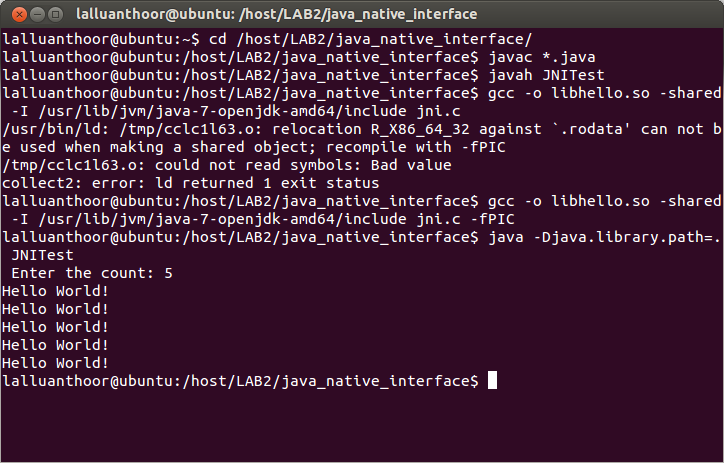
\includegraphics[width=\textwidth]{jni_op.png}
			\caption{Screen-shot of Output}
		\end{figure} 

	%% RESULT IS OBTAINED/SPECIFIED REGARDING THE PROBLEM DEFINITION OR AIM
	\subsection{RESULT}
		\par The k-th largest element of an array was found out and displayed. The scalability and the accuracy of the program were verified.
	
	%% INFERENCE IS OBTAINED/SPECIFIED REGARDING THE OBJECTIVE AND PROCEDURE
	\subsection{INFERENCES}
		\par The selection sort algorithm for sorting elements in descending order can be used to find the k-th largest element. The time complexity of the modified selection sort was found to be $O(n.k)$.

\newpage  %% << END YOUR PROGRAM WITH A 'newpage' COMMAND